\documentclass[italian,a4paper]{article}
\usepackage[tight,nice]{units} %unità di misura
\usepackage{babel,amsmath,amssymb,amsthm,graphicx,url}
\usepackage[text={5.5in,9in},centering]{geometry}
\usepackage[utf8x]{inputenc}
\usepackage[T1]{fontenc}
\usepackage{ae,aecompl}
\usepackage[footnotesize,bf]{caption}
\usepackage[usenames]{color}
\usepackage{textcomp}
\usepackage{gensymb}
\usepackage{pstricks}
\frenchspacing
\pagestyle{plain}
%------------- eliminare prime e ultime linee isolate
\clubpenalty=9999%
\widowpenalty=9999
%--- definizione numerazioni
\renewcommand{\theequation}{\thesection.\arabic{equation}}
\renewcommand{\thefigure}{\arabic{figure}}
\renewcommand{\thetable}{\arabic{table}}
\addto\captionsitalian{%
\renewcommand{\figurename}%
{Grafico}%
}
%
%------------- ridefinizione simbolo per elenchi puntati: en dash
%\renewcommand{\labelitemi}{\textbf{--}}
\renewcommand{\labelenumi}{\textbf{\arabic{enumi}.}}
\setlength{\abovecaptionskip}{\baselineskip}   % 0.5cm as an example
\setlength{\floatsep}{2\baselineskip}
\setlength{\belowcaptionskip}{\baselineskip}   % 0.5cm as an example
%--------- comandi insiemi numeri complessi, naturali, reali e altre abbreviazioni
\renewcommand{\leq}{\leqslant}
%--------- porzione dedicata ai float in una pagina:
\renewcommand{\textfraction}{0.05}
\renewcommand{\topfraction}{0.95}
\renewcommand{\bottomfraction}{0.95}
\renewcommand{\floatpagefraction}{0.35}
\setcounter{totalnumber}{5}
%---------
%
%---------
\begin{document}
\title{Relazione di laboratorio: diodo}
\author{\normalsize Ilaria Brivio (582116)\\%
\normalsize \url{brivio.ilaria@tiscali.it}%
\and %
\normalsize Matteo Abis (584206)\\ %
\normalsize \url{webmaster@latinblog.org}
\and %
\normalsize Lorenzo Rossato (579393)\\ %
\normalsize \url{supergiovane05@hotmail.com}}
\date{\today}
\maketitle
%------------------
\noindent
Sia $V_{\text{in}}$ un segnale:
\begin{table}[h]
    \centering
    \begin{tabular}{rl}
        forma: & triangolare\\
        frequenza: & \unit[123.1]{kHz}\\
        ampiezza pp: & \unit[10]{V}\\
        valor medio: & \unit[0]{V}
    \end{tabular}
\end{table}\\
Dimensionare $R_1$ in modo che la corrente abbia un valore massimo di circa
\unit[5]{mA}.Connettere $V_{\text{in}}$ e $V_{\text{out}}$ ai canali 1 e 2 dell’oscilloscopio
rispettivamente, mediante le sonde. 
Riportare in grafico
l'andamento dell'ingresso e dell'uscita in funzione del tempo per la
durata di un quarto di periodo (grafico~\ref{fig:vinvout}), misurandone i valori allo
stesso istante. Eseguire la misura con particolare cura nella zona
prossima allo zero. Tracciare il grafico della curva caratteristica
(grafico~\ref{fig:cardiodo}).

La frequenza è leggermente maggiore di \unit[100]{kHz} per evitare di dover cambiare scala troppo spesso nel
prendere le misure.  La resistenza R ha valore nominale \unit[1]{k\ohm}. Ovvero \unit[$0.996\pm0.006$]{k\ohm}, misurata con il multimetro T110B, con fondo
scala \unit[2]{k\ohm}.
\begin{figure}[h]
    \begin{center}
        \psset{unit=1in,cornersize=absolute,dimen=middle}%
\begin{pspicture}(-1.395,-0.9625)(0.383333,1.254722)%
% dpic version 16.Jan.09 for PSTricks 0.93a or later
\psset{linewidth=0.8pt}%
\psset{linewidth=0.8pt}%
\makeatletter\@ifundefined{MPSTPatchA}{\def\psbezier@ii{\addto@pscode{%
\ifshowpoints true \else false \fi\tx@OpenBezier%
\ifshowpoints\tx@BezierShowPoints\fi}\end@OpenObj}%
\global\def\MPSTPatchA{}}{}\makeatother%
\psset{arrowsize=1.1pt 4,arrowlength=1.64,arrowinset=0}%
\psline(0,0)(0,0.15)
(0,0.15)(-0.01107,0.15)
\psline(0,0.6)(0,0.45)
(0,0.45)(-0.01107,0.45)
\psline(-0.2,0.2)(-0.2,0.4)
\psline(-0.325,0.3)(-0.2,0.3)
\psline(0,0.15)(-0.2,0.24)
\psline[arrowsize=0.055556in 0,arrowlength=1.5,arrowinset=0]{<-}(-0.05,0.1725)(-0.15,0.2175)
\psline(0,0.45)(-0.2,0.36)
\psline(0,0.6)(0,0.775)
(0,0.775)(-0.041667,0.795833)
(-0.041667,0.795833)(0.041667,0.8375)
(0.041667,0.8375)(-0.041667,0.879167)
(-0.041667,0.879167)(0.041667,0.920833)
(0.041667,0.920833)(-0.041667,0.9625)
(-0.041667,0.9625)(0.041667,1.004167)
(0.041667,1.004167)(0,1.025)
(0,1.025)(0,1.2)
\uput{0.501875ex}[r](0.041667,0.9){\rlap{$ R_c$}}
\pscircle[fillstyle=solid,fillcolor=black](0,0.6){0.02}
\uput{0.501875ex}[r](0.02,0.6){\rlap{$ V_\text{out}$}}
\pscircle[fillstyle=solid,fillcolor=black](0,1.2){0.02}
\uput{0.501875ex}[u](0,1.22){$ +\unit[15]{V}$}
\psline(-0.325,0.3)(-0.775,0.3)
\psline(-0.775,0.3)(-0.775,0.6)
\psline(-0.775,0.6)(-0.775,0.775)
(-0.775,0.775)(-0.816667,0.795833)
(-0.816667,0.795833)(-0.733333,0.8375)
(-0.733333,0.8375)(-0.816667,0.879167)
(-0.816667,0.879167)(-0.733333,0.920833)
(-0.733333,0.920833)(-0.816667,0.9625)
(-0.816667,0.9625)(-0.733333,1.004167)
(-0.733333,1.004167)(-0.775,1.025)
(-0.775,1.025)(-0.775,1.2)
\uput{0.501875ex}[r](-0.733333,0.9){\rlap{$ R_1$}}
\pscircle[fillstyle=solid,fillcolor=black](-0.775,1.2){0.02}
\uput{0.501875ex}[u](-0.775,1.22){$ +\unit[15]{V}$}
\psline(-0.775,0.3)(-0.775,0)
\psline(-0.775,0)(-0.775,-0.325)
(-0.775,-0.325)(-0.733333,-0.345833)
(-0.733333,-0.345833)(-0.816667,-0.3875)
(-0.816667,-0.3875)(-0.733333,-0.429167)
(-0.733333,-0.429167)(-0.816667,-0.470833)
(-0.816667,-0.470833)(-0.733333,-0.5125)
(-0.733333,-0.5125)(-0.816667,-0.554167)
(-0.816667,-0.554167)(-0.775,-0.575)
(-0.775,-0.575)(-0.775,-0.9)
\uput{0.501875ex}[r](-0.733333,-0.45){\rlap{$ R_2$}}
\psline(-0.691667,-0.9)(-0.858333,-0.9)
\psline(-0.719444,-0.93125)(-0.830556,-0.93125)
\psline(-0.739286,-0.9625)(-0.810714,-0.9625)
\psline(-0.775,0.3)(-1.05,0.3)
\psline(-1.05,0.383333)(-1.05,0.216667)
\psline(-1.1,0.383333)(-1.1,0.216667)
\psline(-1.1,0.3)(-1.375,0.3)
\uput{0.501875ex}[u](-1.075,0.383333){$ C_1$}
\pscircle[fillstyle=solid,fillcolor=black](-1.375,0.3){0.02}
\uput{0.501875ex}[d](-1.375,0.28){$ V_\text{in}$}
\psline(0,0)(-0,-0.1)
(-0,-0.1)(0.041667,-0.120833)
(0.041667,-0.120833)(-0.041667,-0.1625)
(-0.041667,-0.1625)(0.041667,-0.204167)
(0.041667,-0.204167)(-0.041667,-0.245833)
(-0.041667,-0.245833)(0.041667,-0.2875)
(0.041667,-0.2875)(-0.041667,-0.329167)
(-0.041667,-0.329167)(0,-0.35)
(0,-0.35)(0,-0.45)
\uput{0.501875ex}[l](-0.125,-0.225){\llap{$ R_{e1}$}}
\psline(0,-0.45)(-0,-0.55)
(-0,-0.55)(0.041667,-0.570833)
(0.041667,-0.570833)(-0.041667,-0.6125)
(-0.041667,-0.6125)(0.041667,-0.654167)
(0.041667,-0.654167)(-0.041667,-0.695833)
(-0.041667,-0.695833)(0.041667,-0.7375)
(0.041667,-0.7375)(-0.041667,-0.779167)
(-0.041667,-0.779167)(0,-0.8)
(0,-0.8)(0,-0.9)
\uput{0.501875ex}[l](-0.125,-0.675){\llap{$ R_{e2}$}}
\psline(0.083333,-0.9)(-0.083333,-0.9)
\psline(0.055556,-0.93125)(-0.055556,-0.93125)
\psline(0.035714,-0.9625)(-0.035714,-0.9625)
\psline(0,-0.45)(0.3,-0.45)
\psline(0.3,-0.45)(0.3,-0.65)
\psline(0.216667,-0.65)(0.383333,-0.65)
\psline(0.216667,-0.7)(0.383333,-0.7)
\psline(0.3,-0.7)(0.3,-0.9)
\uput{0.501875ex}[ur](0.325,-0.675){\rlap{$ C_2$}}
\psline(0.383333,-0.9)(0.216667,-0.9)
\psline(0.355556,-0.93125)(0.244444,-0.93125)
\psline(0.335714,-0.9625)(0.264286,-0.9625)
\end{pspicture}%

    \end{center}
\end{figure}\\
Le barre di errore sui grafici rappresentano l'accuratezza delle misure,
determinate dalle specifiche tecniche dell'oscilloscopio. In particolare:
Queste incertezze sono propagate linearmente alla corrente e differenza di
potenziale attraverso il diodo:
\begin{align*}
    I_d &= \dfrac{V_{\text{out}}}{R}\\
    \dfrac{\Delta{I_d}}{I_d} &= \left(\dfrac{\Delta R}{R}\right) + \left(\dfrac{\Delta
    V_\text{out}}{V_\text{out}}\right) = 3.05\%\\
    \dfrac{\Delta{V_d}}{V_d} &= 3\%\\
\end{align*}  
\newpage
\section{Appendice: tabelle e grafici}
\begin{table}[h]\caption{Dati raccolti nel quarto di periodo dell'onda
    triangolare. Sono riportati anche nel seguente
    grafico~\ref{fig:vinvout}}\label{tab:vinvout}
    \centering
    \begin{tabular}{*3c}
t (ns) &   $V_{\text{in}}$ (V) &  $V_{\text{out}}$ (V)\\\hline
\multicolumn{3}{c}{scala t = 250ns, V = 1 V}\\
2080&   4.44&   3.60\\
2000&   4.32&   3.48\\
1750&   3.80&   2.96\\
1500&   3.28&   2.48\\
1250&   2.72&   1.96\\
1000&   2.20&   1.48\\
750&    1.68&   1.00\\
500&    1.12&   0.48\\\hline 
\multicolumn{3}{c}{scala t = \unit[100]{ns}, V = \unit[0.2]{V}}\\
700&    1.54&   0.872\\
600&    1.35&   0.680\\
500&    1.14&   0.488\\
400&    0.920&  0.304\\
300&    0.696&  0.128\\
200&    0.472&  0.016\\\hline  
\multicolumn{3}{c}{scala t = \unit[50]{ns}, V = \unit[0.05]{V}}\\
150&    0.346&  0.004\\
100&    0.234&  0.000\\
50&0.118&  0.000
\end{tabular}
\end{table}
\begin{table}[p]\caption{Dati nel grafico~\ref{fig:cardiodo}. Differenza di
    potenziale ai capi del diodo e intensità di corrente calcolate, con i
    rispettivi errori.}\label{tab:cardiodo}
        \centering
        \begin{tabular}{r@{ $\pm$ }l r@{ $\pm$ }l}
                \multicolumn{2}{c}{$V_d$ (\unit{V})} &
                \multicolumn{2}{c}{$I_d$ (\unit{mA})} \\\hline
                0.84 & 0.03 & 3.60 & 0.13\\
                0.84 & 0.03 & 3.48 & 0.13\\
                0.84 & 0.03 & 2.96 & 0.11\\
                0.80 & 0.02 & 2.48 & 0.09\\
                0.76 & 0.02 & 1.96 & 0.07\\
                0.72 & 0.02 & 1.48 & 0.05\\
                0.68 & 0.02 & 1.00 & 0.04\\
                0.64 & 0.02 & 0.48 & 0.02\\
                0.67 & 0.02 & 0.87 & 0.03\\
                0.67 & 0.02 & 0.68 & 0.02\\
                0.65 & 0.02 & 0.49 & 0.02\\
                0.62 & 0.02 & 0.30 & 0.01\\
                0.57 & 0.02 & 0.131 & 0.004\\
                0.46 & 0.01 & 0.020 & 0.001\\
                0.34 & 0.01 & 0.000 & 0.000\\
                0.23 & 0.01 & 0.000 & 0.000\\
                0.122 & 0.003 & 0.000 & 0.000\\
            \end{tabular}
                \end{table}

\begin{figure}[p]\caption{Andamento di $V_\text{in}$ ($\times$) e
    $V_\text{out}$ ($+$) per un quarto di periodo, tempo in nanosecondi e
    potenziale in Volt. I dati fanno riferimento alla
    tabella~\ref{tab:vinvout}} 
    \centering
    \includegraphics[angle=-90,width=\textwidth]{diodo.ps}\label{fig:vinvout}
\end{figure}
\begin{figure}[p]\caption{Curva caratteristica del diodo, con $V_d$ in
    ascissa (V) e $I_d$ in ordinata (\unit{mA}). I dati fanno riferimento
    alla tabella~\ref{tab:cardiodo}.} 
    \centering
    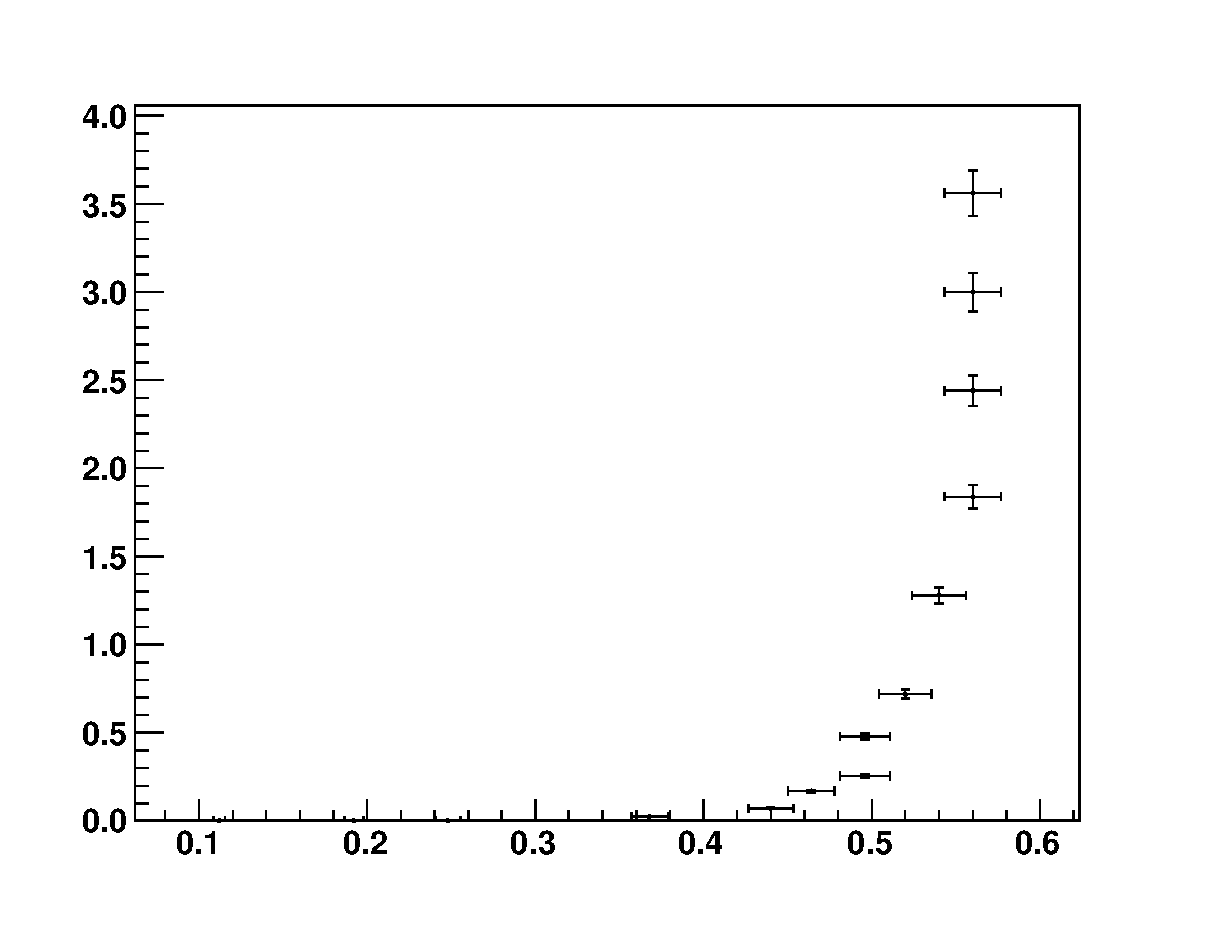
\includegraphics[width=\textwidth]{car.eps}\label{fig:cardiodo}
\end{figure}
\end{document}


